\begin{enumerate}
    \item
	\begin{itemize}
	    \item Percentage of population that is of hispanic heritage (racePctHisp): Hispanic is a race term with a meaning that has historically been changed as a result of policy decisions.  
	    \item Number of people living in areas classified as urban (numbUrban): Urban is a term with a meaning that has changed as a result of policy decisions.
	    \item Percentage of people under the poverty level (PctPopUnderPov): Poverty level has changed as a result of policy decisions.
	\end{itemize}
    \item
	\begin{itemize}
	    \item Percentage of males who are divorced (MalePctDivorce): It might be assumed that higher rates of divorce cause higher crime rates but it could also be the case that higher crime rates case in an area cause higher divorce rates.
	    \item Number of vacant households (HousVacant): It might be assumed that more vacant housholds cause higher crime rates but it could also be the case that higher crime rates cause there to be more vacant houses. 
	    \item Number of homeless people counted in the street (NumStreet): It might be assumed that more homeless people in the street cause higher crime rates but it could also be the case that higher crime rates cause there to be more homeless people in the street.
	\end{itemize}
\end{enumerate}

\begin{enumerate}
    \item See Figure 3.
	\begin{figure}[h!]
	    \centering
	    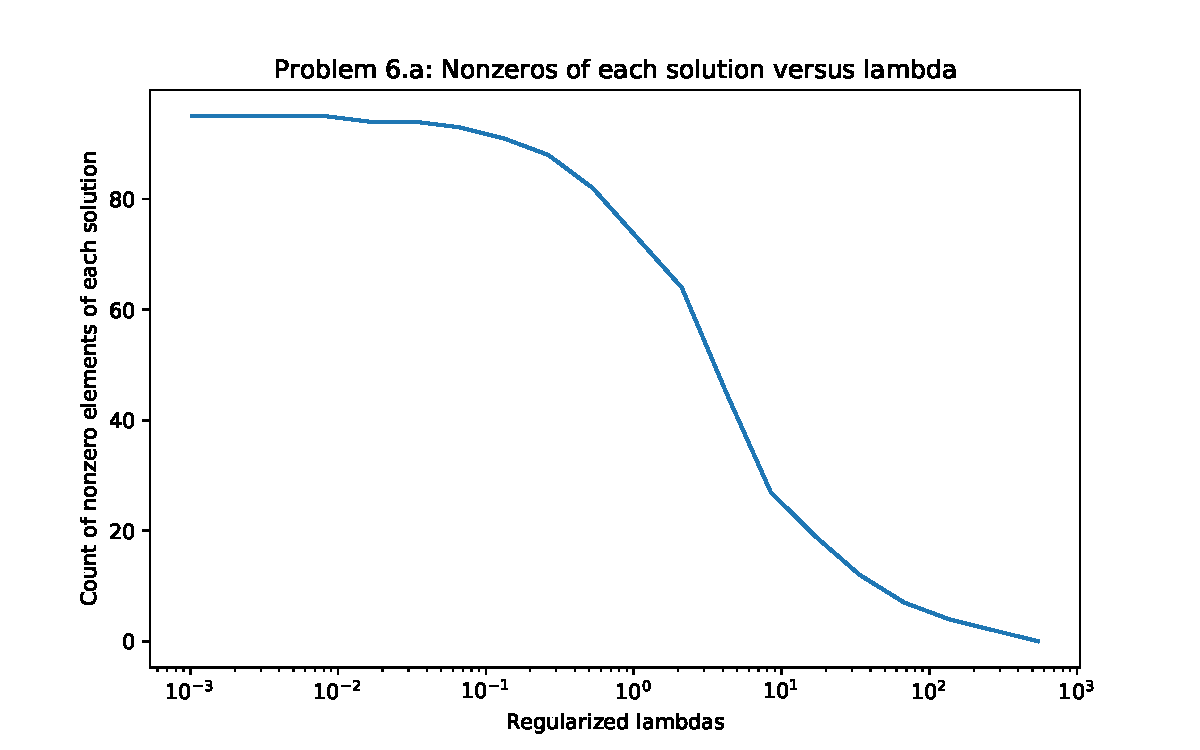
\includegraphics[width=0.5\linewidth]{images/P6_a.pdf}
	    \caption{}
	\end{figure}
    \item See Figure 4.
	\begin{figure}[h!]
	    \centering
	    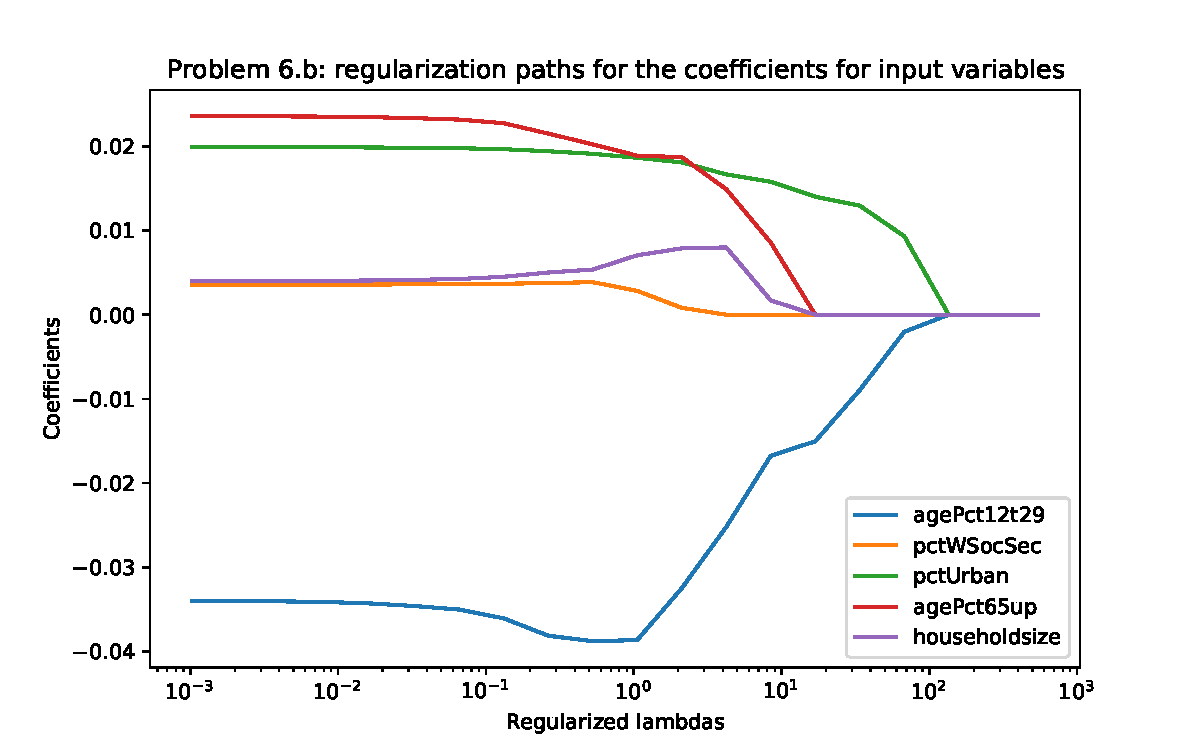
\includegraphics[width=0.5\linewidth]{images/P6_b.pdf}
	    \caption{}
	\end{figure}

    \item See Figure 5.
	\begin{figure}[h!]
	    \centering
	    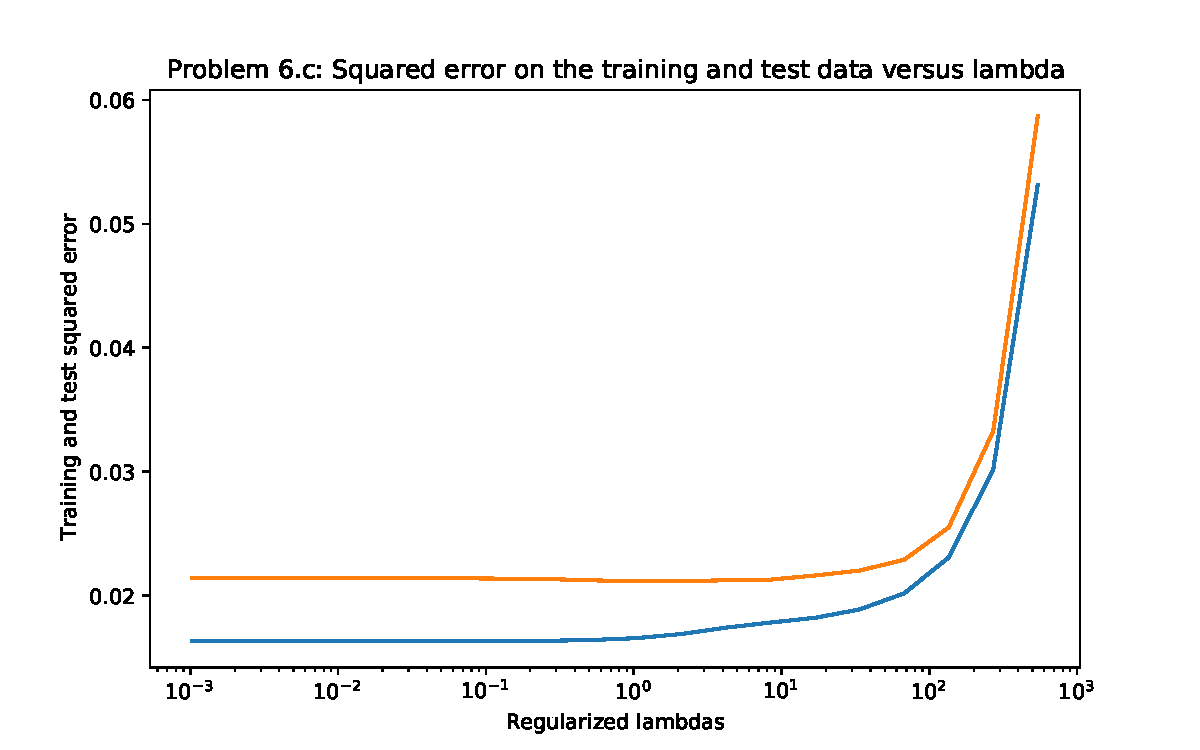
\includegraphics[width=0.5\linewidth]{images/P6_c.pdf}
	    \caption{}
	\end{figure}
    \item See Figure 6. \\
	Minimum weight: index 39, PctKids2Par with value -0.1247.\\
	Maximum weight: index 45, PctIlleg with value 0.0687.\\
	Crime rates correlate most positively with ``percentage of kids born to never married'' (PctIlleg) and correlate most negatively with ``percentage of kids in family housing with 2 parents'' (PctKids2Par). These data suggest that crime rates increase with increases in percentage of kids born to never married and decrease with increases in percentage of kids in family housing with 2 parents.
	\begin{figure}[h!]
	    \centering
	    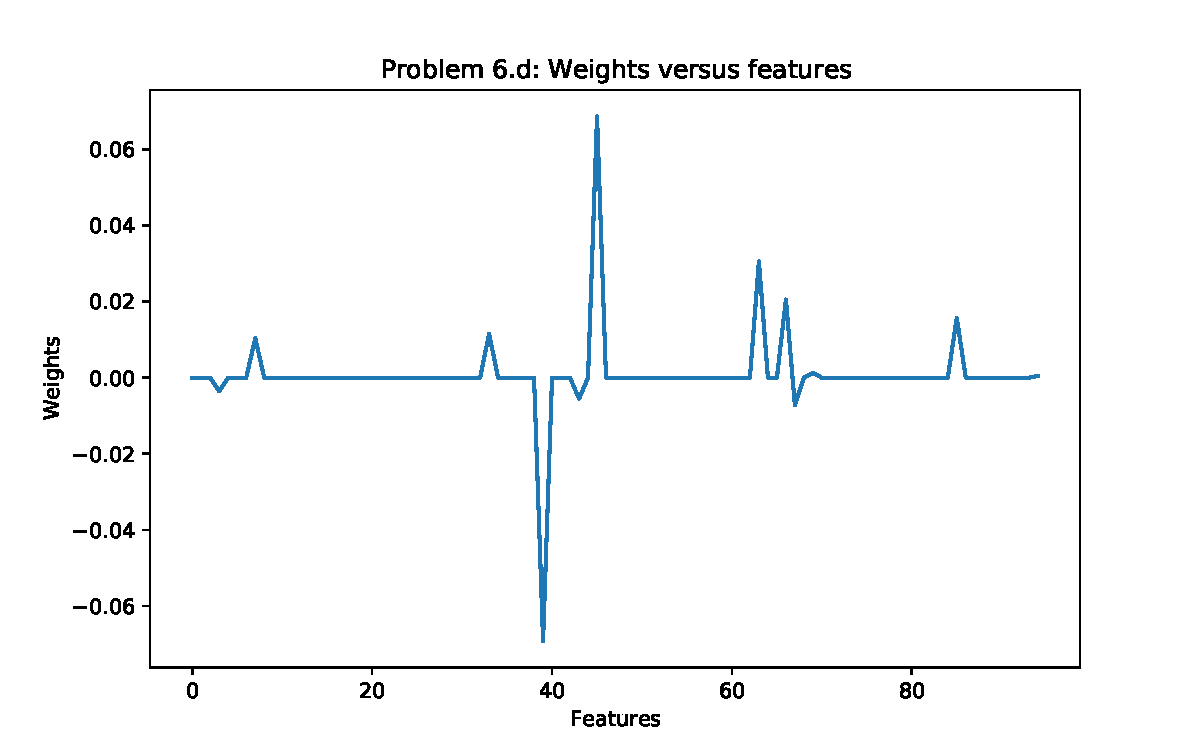
\includegraphics[width=0.5\linewidth]{images/P6_d.pdf}
	    \caption{}
	\end{figure}
    \item The dictum that "Correlation does not equal Causation" holds. More over-65 years old people living in an area doesn't cause lower crime rates. There are many confounding factors. One could be that older people move away from high crime rate areas. So rather than there presence indicating low crime rates their absence can indicate high crime rates. And, should older people return, the crime rates could remain the same, or even increase, if we assume that older people are more likely to be targeted by criminals than younger people. 
\end{enumerate}
